\newpage
\section{System Databases}

Needs an introductory paragraph here.

\subsection{MagicDraw}

MagicDraw \citep{MagicDraw-cite} is a tool used by the project to maintain a model of the Rubin Observatory system creating a relational database between system elements.  Developed through the Rubin Observatory's use of MagicDraw, user guides are collected on the following Project confluence page: \href{https://confluence.lsstcorp.org/display/SYSENG/MagicDraw+LSST+Users+Guide}{MagicDraw Users Guide}.

The system elements captured with the MagicDraw database include:

\begin{itemize}
	\item Hazard Analysis - imported from various vendor and internal spreadsheets and now source of truth. Synced to Jira for verification
	\item FMEA - imported from various vendor and internal spreadsheets and now source of truth (currently incomplete)
	\item Requirements - source of truth with exports to DocuShare
	\item Verification Elements - source of truth for requirements details, synced to/from Jira
	\item Verification Plans/Cycles/Cases - synced to/from Jira, not source of truth
	\item SAL Commands, Events, Telemetry - imported from CSC XML
	\item Operations Concepts - source of truth
	\item System level state machine - source of truth
	\item Interlocks - modeled from source material
	\item Structural decomposition - sync from SolidWorks in the future
\end{itemize}

\subsection{JIRA}

JIRA is used by the by the Construction Project for many purposes.  JIRA is primarily a issue tracking tool where teams/groups can document, organize, track and report on software or administrative tasks. \citep{JIRA-cite} The tool is organized in "work spaces" called projects, each of which tracks a list of enumerated tickets or issues. JIRA provides a wide variety of tools to manipulate or organize projects and tickets. Many of these projects are very specialized or have been set up for personal use.  Listed below are projects related to the deliverables from the integrated Rubin Construction Project spanning of two independent repositories - one served out of Tucson for the MREFC effort and another served out of SLAC for the DOE MIE LSSTCam effort.

Need introductory/summary paragraph here about Tucson-based JIRA Projects.

\begin{itemize}
	\item Verification Elements/Plans/Cycles/Cases/Results - source of truth
	\item Risks, Opportunities, Mitigations - source of truth
	\item FRACAS - Failures, corrective actions - source of truth
	\item Hazard mitigation verification
\end{itemize}

Need introductory/summary paragraph here about LSSTCam-based JIRA Projects.
The list below collects JIRA projects within the SLAC-based JIRA instance. These items require SLAC LSSTCam credentials.

\begin{itemize}
	\item \href{https://jira.slac.stanford.edu/browse/LCAI}{Camera Action Items}: Captures action items for all Camera Subsystems, from various sources (reviews, internal discussions, etc.). Utilization is described on this confluence page: \href{https://confluence.slac.stanford.edu/pages/viewpage.action?pageId=130884357}{Using JIRA and Confluence to track Action Items}.
	\item \href{https://jira.slac.stanford.edu/browse/LSSTTD}{Test Data Framework}:  Spans many purposes, includes (not exclusive) reporting \href{http://lsst-camera.slac.stanford.edu/DataPortal/}{Data Portal}, \href{http://srs.slac.stanford.edu/DataCatalog/?experiment=LSST-CAMERA}{Data Catalog}, CCS initiated analyses, limitations, improvements (web-app or otherwise), eTraveler or database impacts (typically data structure related or new implementations).
	\item Camera Control System Core
	\begin{itemize}
		\item \href{https://jira.slac.stanford.edu/browse/LSSTCCS}{CCS Core}:  Self-explanatory.
		\item \href{https://jira.slac.stanford.edu/browse/LSSTCCSDRIVER}{CCS Driver}:  Driver development for using specific software/equipment with CCS.
		\item \href{https://jira.slac.stanford.edu/browse/LSSTCCSSUB}{CCS Subsystem}:   Not sure the difference between this and CCS Core.
		\item \href{https://jira.slac.stanford.edu/browse/LSSTCCSPROJ}{CCS Project}:  Old project; as stated by \href{https://jira.slac.stanford.edu/browse/LSSTCCSPROJ-80}{LSSTCCSPROJ-80}, it is replaced by CCS Core; but unsure if all tickets were migrated (open or closed).
		\item \href{https://jira.slac.stanford.edu/browse/LSSTCCSDOC}{CCS Documentation}:  Old project, few tickets remain open.
	\end{itemize}
	\item CCS Camera Subsystem and Interfaces Related
		\begin{itemize}
		\item \href{https://jira.slac.stanford.edu/browse/LSSTCCSPOWER}{CCS Power Manager Subsystem}:  self-explanatory.
		\item \href{https://jira.slac.stanford.edu/browse/LSSTCCSRAFTS}{CCS Rafts}:  self-explanatory.
		\item \href{https://jira.slac.stanford.edu/browse/LSSTCCSREFRIG}{CCS Refrigerator}:  self-explanatory.
		\item \href{https://jira.slac.stanford.edu/browse/LSSTCCSSHUTTER}{CCS Shutter}:  self-explanatory.
		\item \href{https://jira.slac.stanford.edu/browse/LSSTCCSUT}{CCS Utility Trunk}:  self-explanatory.
		\item \href{https://jira.slac.stanford.edu/browse/LCOBM}{CCS OCS Bridge and MCM}:  self-explanatory.
		\item \href{https://jira.slac.stanford.edu/browse/LSSTCCSDAQ}{CCS DAQ}:  self-explanatory.
		\item \href{https://jira.slac.stanford.edu/browse/LSSTCCSFCS}{CCS FCS}:  self-explanatory (FCS - filter change system?).	
	\end{itemize}
	\item CCS and Specific Applications
	\begin{itemize}
		\item \href{https://jira.slac.stanford.edu/browse/LSSTCCSTS}{CCS Test Stands}:  use of and item-specific items for test stands at various sites.
		\item \href{https://jira.slac.stanford.edu/browse/LSSTIR}{CCS IR2 Infrastructure}:  self-explanatory (IR2 is the SLAC Cleanroom).
		\item \href{https://jira.slac.stanford.edu/browse/LSSTCCSCOM}{CCS ComCam}:  self-explanatory, but issues not exclusive to this JIRA project.
	\end{itemize}
	\item \href{https://jira.slac.stanford.edu/browse/LSSTDREB}{DREB Firmware}:  8 tickets (all resolved) for DREB.
	\item \href{https://jira.slac.stanford.edu/browse/ETCCB}{eTraveler CCB}:  Changes to instructions, local software changes (Job Harness/Install), and a few decisions about how eTraveler was organized/implemented (software and hardware). See the following confluence page for context on CCB use: \href{https://confluence.slac.stanford.edu/display/LSSTCAM/eTraveler+CCB}{eTraveler CCB}
\end{itemize}

\subsection{Drupal}

Rubin uses the Drupal web content management framework as its websites’ back-end. This includes lsst.org, project.lsst.org and sites created to facilitate project meetings and reviews. To avoid the complication of having to make multiple site updates when content changes, lsst.org and project.lsst.org documents are served by hyperlinks that pull files from whatever repositories contain their sources of truth. While it is possible to upload discrete files to a specific site’s server location, by policy and standard the project eschews doing so, except in the case of meetings and reviews. Those sites’ server directories contain document and presentation files in order to preserve the state of that documentation as it was presented at the time of the meeting or review. However, during or at the conclusion of the event, the files are uploaded to DocuShare in a collection specific to the event. Presentations are uploaded as discrete handles. Other documentation such as policies, requirements, and design documents are uploaded as a zip archive, since they represent a snap-shot of an existing handle. The previous is true for project-level reviews and meetings like the Project and Community Workshops, but it may not be true for Drupal sites used for subsystem-level reviews and workshops.

\begin{itemize}
	\item Change Control What resides in Drupal that is not in DocuShare?
	\item Review materials
	\item Are the review material fully captured in Docushare?  Yes, for Project level reviews.
	\item Open question regarding lower level reviews.
	\item Historical WEB pages
\end{itemize}

\subsection{Euporie}

Euporie is a server in the Rubin construction project network that contains a directory labeled “TS-Deliverables”. The directory contains subfolders of each of the Rubin observatory subsystems being managed by the telescope and site group. The subdirectories contain vendor supplied documentation as contract deliverables (design documentation, construction drawings, manuals and misc. information) for storage.

The Euporie repository can be accessed here (requires Rubin Observatory credentials through VPN): \url{smb://euporie}.

\begin{figure}
\begin{center}
  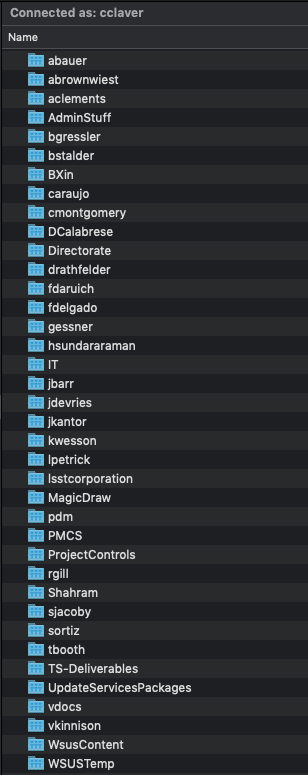
\includegraphics[scale=0.5]{Figures/EuporieDirectory.png}
\end{center}
\caption{\label{fig:EuporyDirectory} The current (June 2021) directory structure of the Euporie remote drive repository}
\end{figure}

\begin{figure}
\begin{center}
  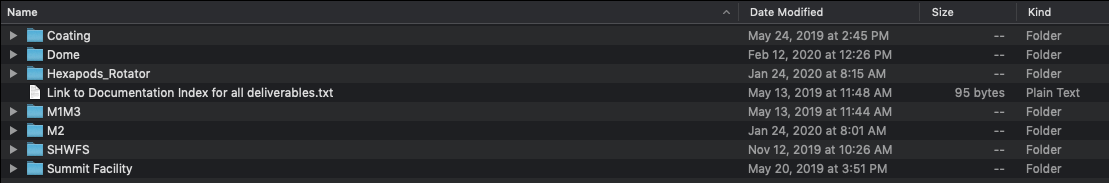
\includegraphics[scale=0.33]{Figures/EuporieTS.png}
\end{center}
\caption{\label{fig:EuporyTS} The Telescope \& Site folders on the Euporie repository used to collect documents from vendors}
\end{figure}

\subsection{T\&S Commandable SAL Component XML Files}

The T\&S XML package defines the data objects for all Commandable SAL Components (CSC). These data objects are defined in XML. SAL consumes the XML to produce language specific libraries that enable communication over the DDS network.  These XML files are critical for defining the configuration and interaction of the systems within the Summit Facility observing environment.

A link to the T\&S TechNote covering the XML files is here: \url{https://ts-xml.lsst.io}

\subsection{LSSTCam}
	\subsubsection{eTraveler}
	eTraveler is a web-based tool used across multiple sites during the testing and construction of the Camera and its subcomponents. It was used to provide procedures, begin testing and data collection locally, upload information and data to servers (primarily to the \href{http://lsst-camera.slac.stanford.edu/DataPortal/}{Data Portal} and \href{http://srs.slac.stanford.edu/DataCatalog/?experiment=LSST-CAMERA}{Data Catalog}), track component/assembly information, and track the acceptance and non-conformance reports.
	
	eTraveler, Data Portal and Data Catalog include independent "prod" and "dev" instances, both of which have information on production parts.
	
	\begin{itemize}
		\item eTraveler: includes \href{https://lsst-camera.slac.stanford.edu/eTraveler/exp/LSST-CAMERA/welcome.jsp?dataSourceMode=Prod}{PROD database} and \href{https://lsst-camera.slac.stanford.edu/eTraveler/exp/LSST-CAMERA/welcome.jsp?dataSourceMode=Dev}{DEV database}
		\item Data Portal: includes \href{https://lsst-camera.slac.stanford.edu/DataPortal/index.jsp?dataSourceMode=Prod}{PROD database} and \href{https://lsst-camera.slac.stanford.edu/DataPortal/index.jsp?dataSourceMode=Dev}{DEV database}
		\item Data Catalog: includes \href{https://srs.slac.stanford.edu/DataCatalog/index.jsp?dataSourceMode=Prod}{PROD database} and \href{https://srs.slac.stanford.edu/DataCatalog/index.jsp?dataSourceMode=Dev}{DEV database}
		\begin{itemize}
			\item Data Portal is user interface and report generation using Data Catalog files/pointers.
			\item \href{https://lsst-camera.slac.stanford.edu/DataPortal/ncrStatus-compact.jsp}{Comprehensive view/search for NCRs}
			\item Some travelers in eTraveler have special reports generated for sensors and rafts, indexed by Run Number.
			\item \href{https://lsst-camera.slac.stanford.edu/DataPortal/aspicStatus.jsp}{ASPIC summary table}
			\item \href{https://lsst-camera.slac.stanford.edu/DataPortal/SensorAcceptance.jsp}{Sensor Acceptance from vendors summary table}
		\end{itemize}
		\item \href{http://dbweb0.fnal.gov/ECL/lsst_camera}{e-log}: possible content, mostly BNL activities. Data not migrated from Fermi Lab server/database. A lot of what used to be in e-log is now in Slack.
		\item Main Content of eTraveler:
		\begin{itemize}
			\item Historical information about how camera was assembled, including specific operators, date/time, results, etc. Some procedures have been moved to DocuShare; unsure of percentage or locations.
			\item Non-conformance reports (NCR) for hardware and operations.
			\item Raw Data and analysis results from test stands (including BNL and IN2P3) and data from BOT/CCOB testing. The data itself is stored at SLAC outside of the eTraveler/DataCatalog database. Much of the data (but not all) has been archived at NCSA.
			\item CCD vendor data (metrology and electro-optical testing) along with the analysis results.
			\item REB testing results from SLAC; and ASPIC testing results before assembly on REB.
			\item Records for acceptance of hardware; most notably sensor acceptance from vendors and Camera subsystem hardware from subsystems (e.g., science and corner rafts).
			\item Records for summary information, e.g. sensor acceptance, pre-ship review of science rafts from BNL to SLAC.
			\item Labels of hardware or travelers capturing specifics or issues.
			\item Hardware inventory tracking, including quantity, location, stock and status.
		\end{itemize}
	\end{itemize}
	\subsubsection{CCS IR2 Database}
	This contains historical telemetry data from all operations (full camera and test stands) in IR2. In addition this contains the "image database" for images taken in the SLAC cleanroom.
	\subsubsection{CCS Summit Database}
	This database contains the following:
	\begin{itemize}
		\item Telemetry from ComCam, Main Camera and Auxiliary Telescope on the summit (in principle also all in EFD)
		\item Configuration for ComCam, Main Camera and Auxiliary Telescope on the summit (in principle all data is in EFD)
		\item Camera Image database for ComCam, Main Camera, Auxiliary Telescope
	\end{itemize}

	\subsubsection{SLAC V--Drive}
	
	\subsubsection{BNL Raft Share Folder}
	A network folder at BNL includes notes, photographs, documents, reports, etc. A large majority of, if not all, critical items should already be in DocuShare, Confluence or eTraveler. The network folder includes historical records, as well.
	
\subsection{Engineering Facility Database}

\subsection{Primavera P6}

\subsection{Miscellaneous}
\begin{itemize}
	\item IN2P3 filter changer documentation: https://filterchangerdoc.pages.in2p3.fr/fcs-doc/
	\item Von Ardenne Catalog: https://vacatalog.vonardenne.biz/index.php/m/home/index
\end{itemize}
